\appendix
\bibliographystyle{IEEEtran}
\bibliography{svp}
\chapter{Images}
\label{apendix:img_transformations}
\begin{figure}
    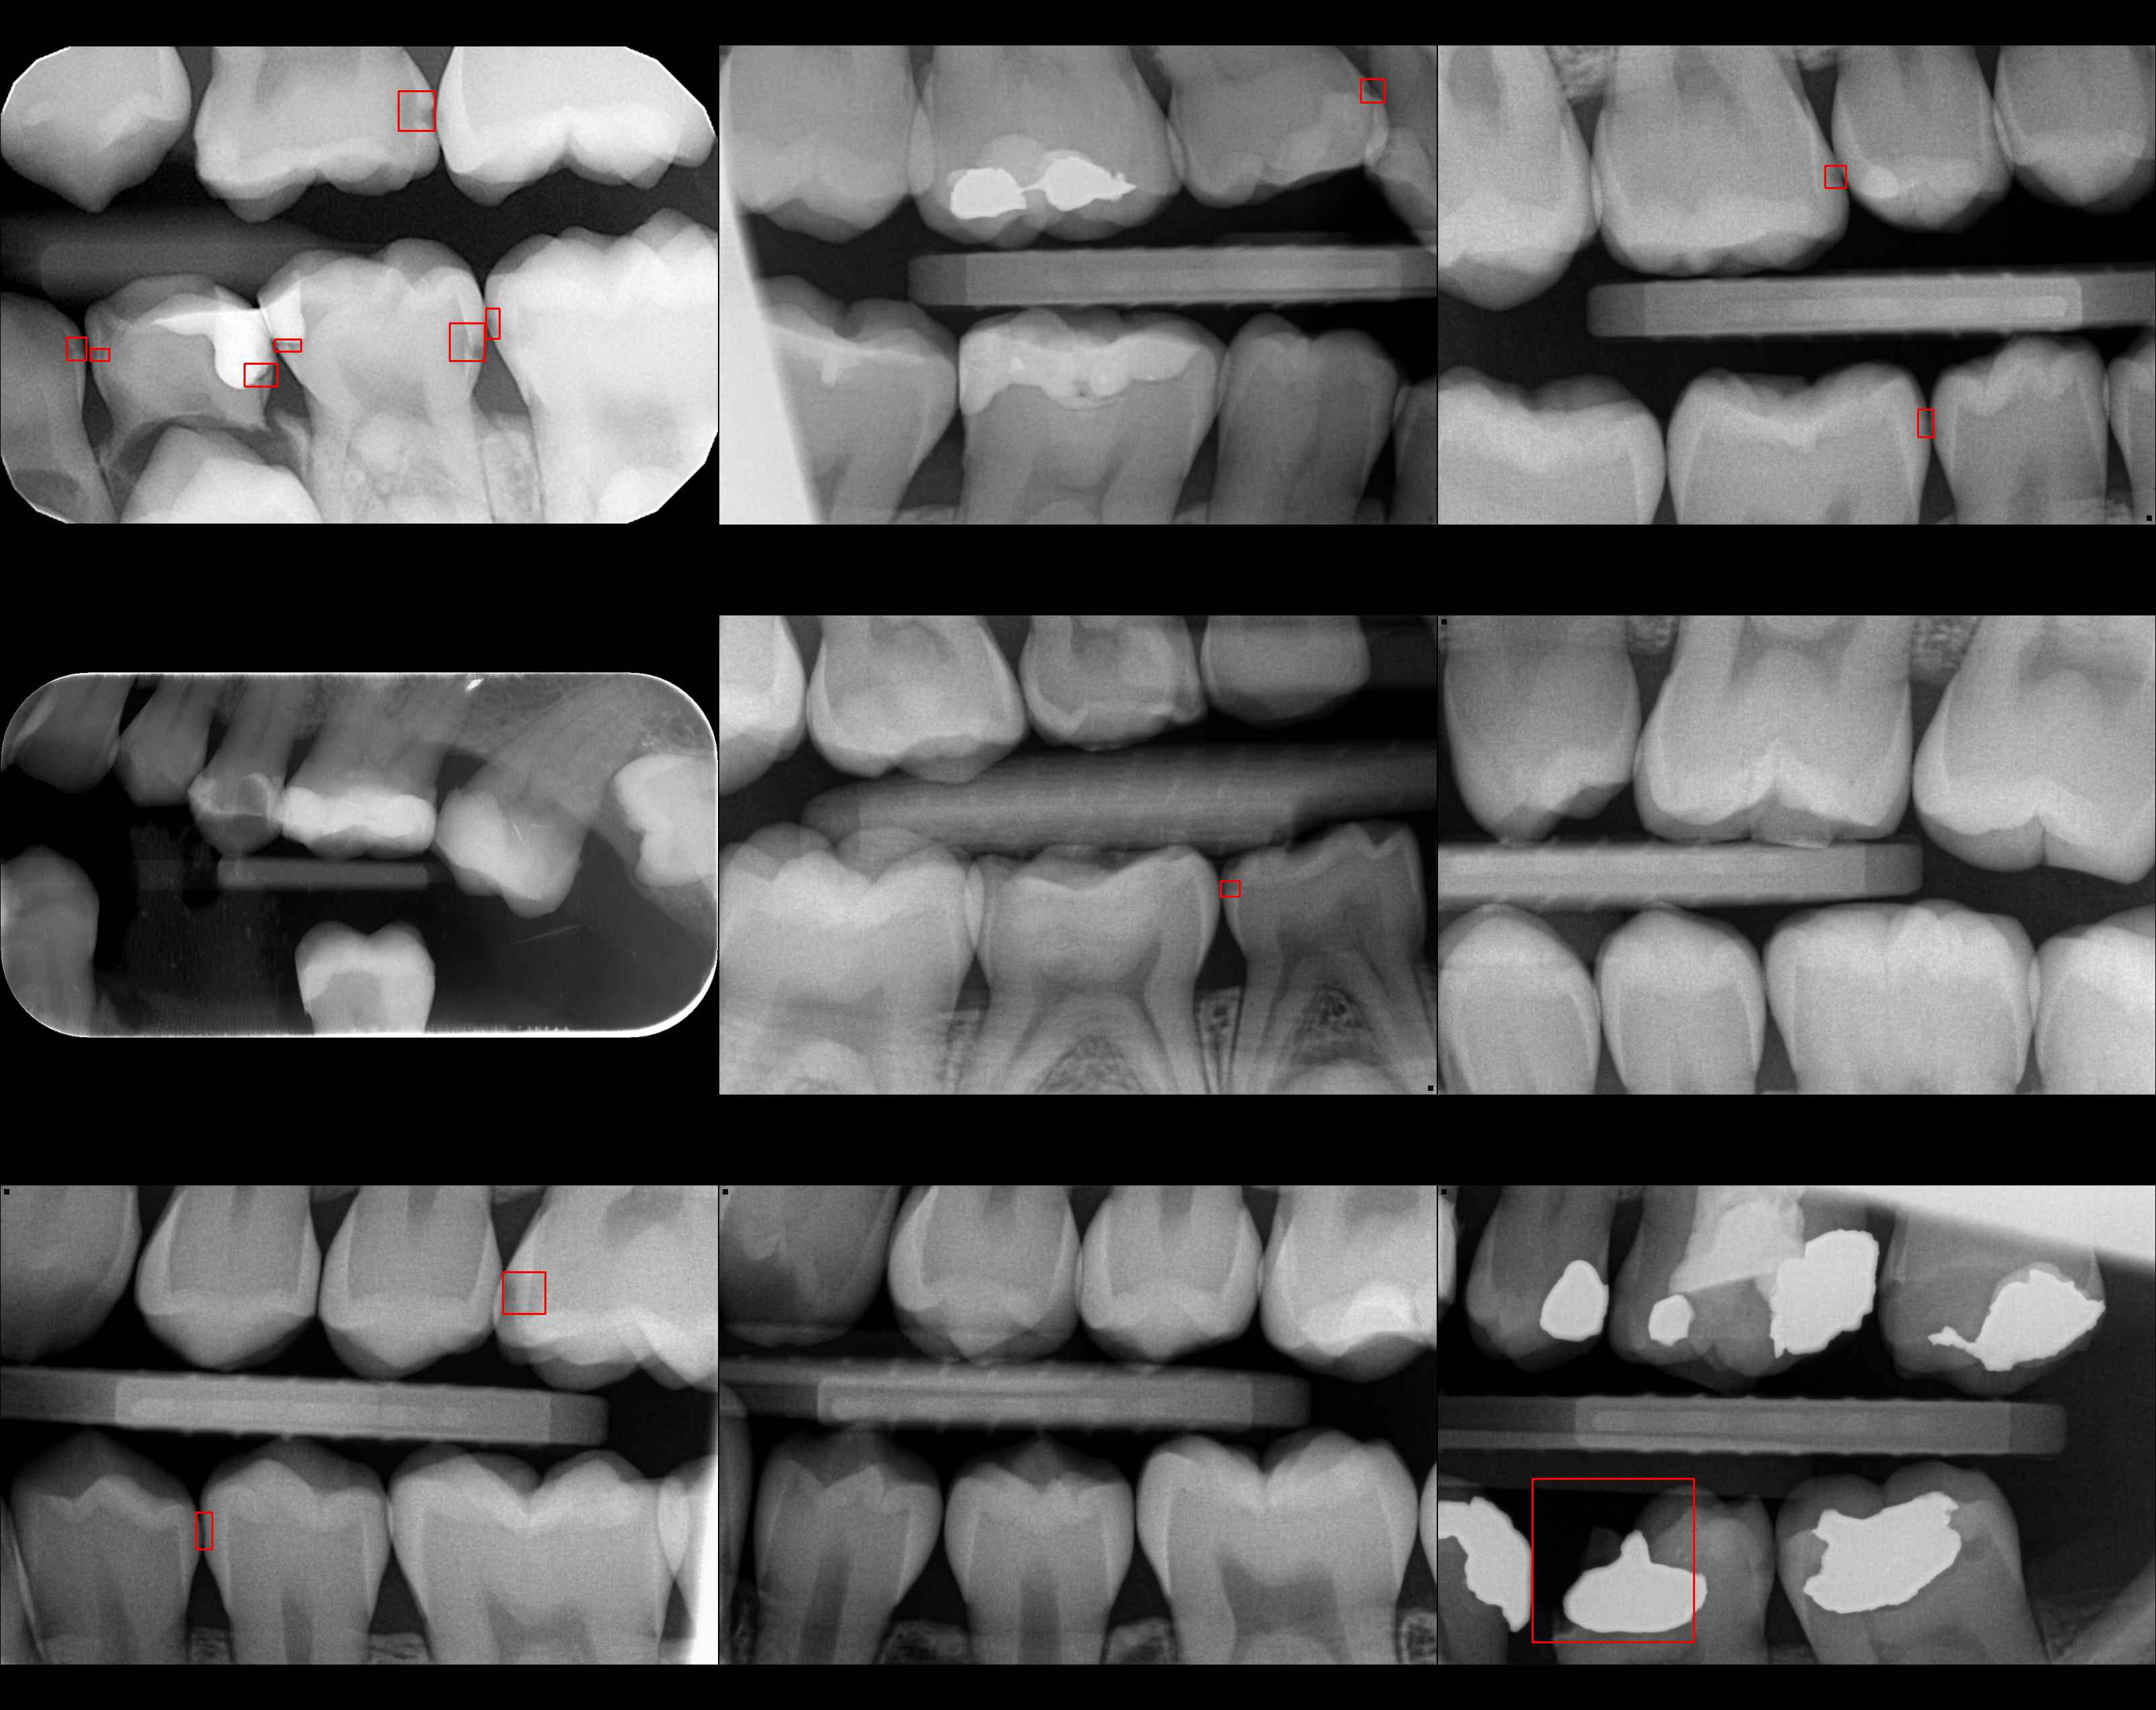
\includegraphics[width =0.9\linewidth]{images/no_trasnforms.jpg}
    \caption{No transformation applied}
\end{figure}
\begin{figure}
    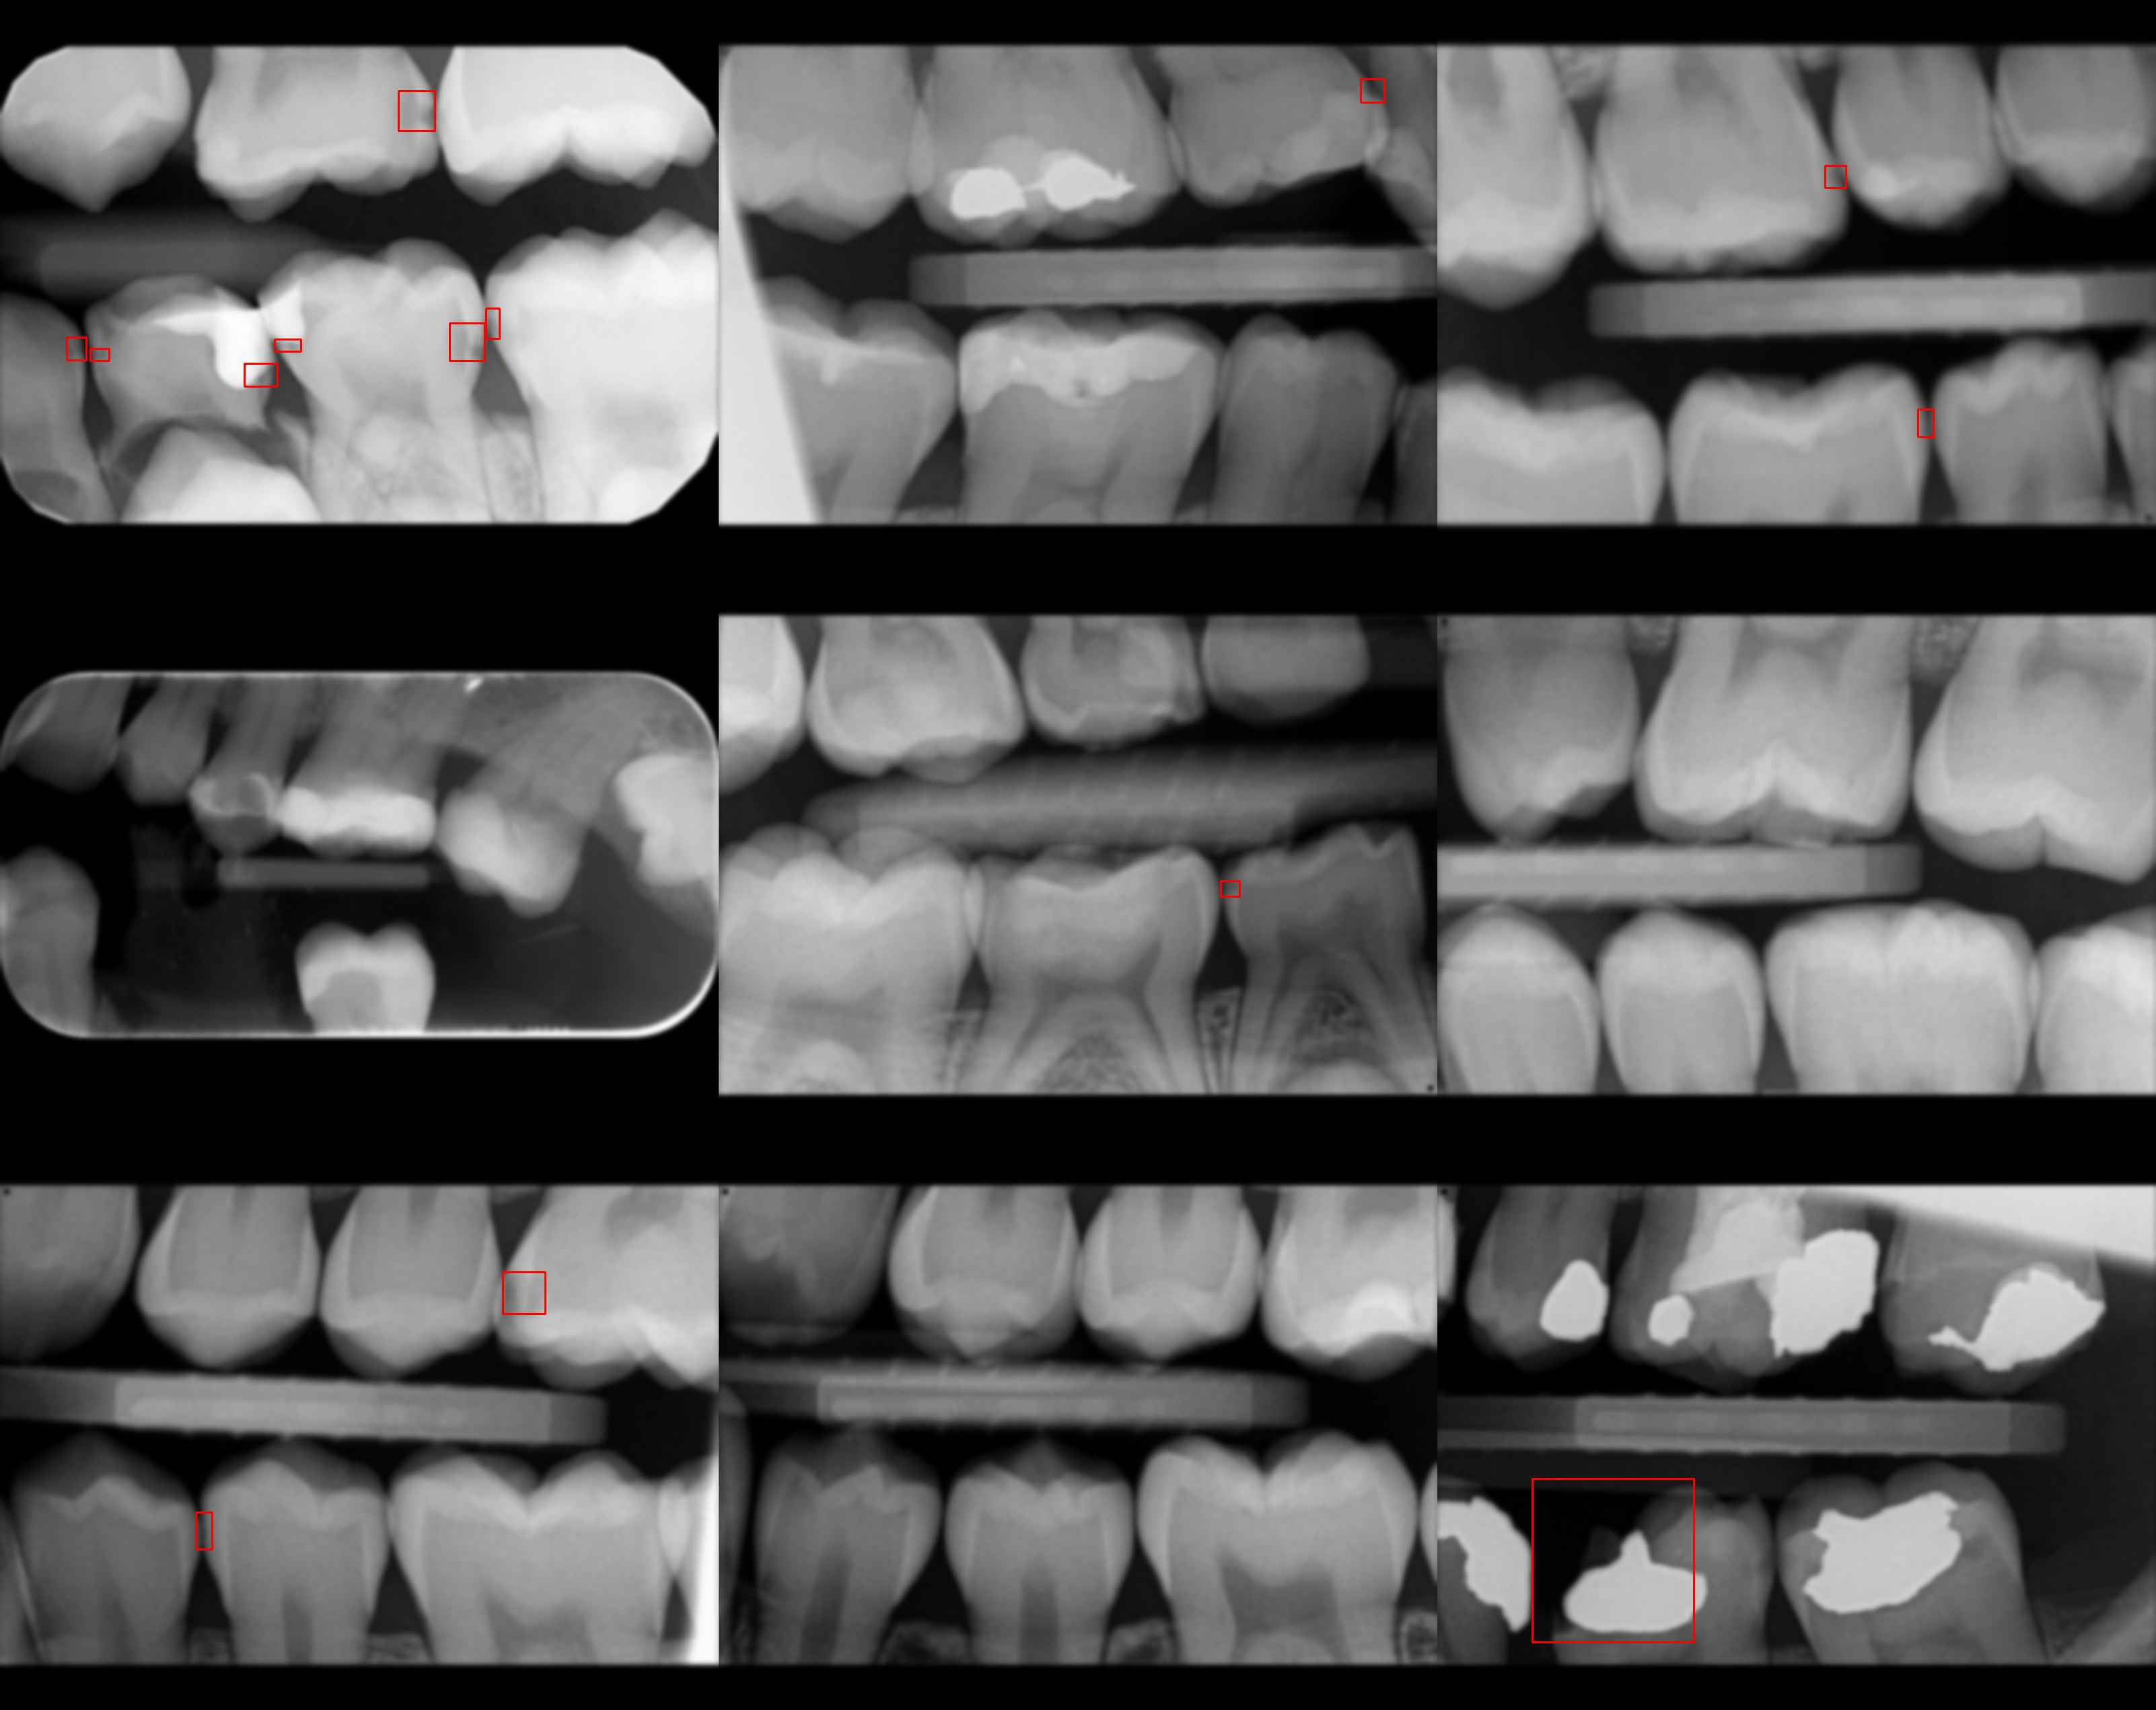
\includegraphics[width =0.9\linewidth]{images/gaussian_blur.jpg}
    \caption{Gaussian blur applied}
\end{figure}
\begin{figure}
    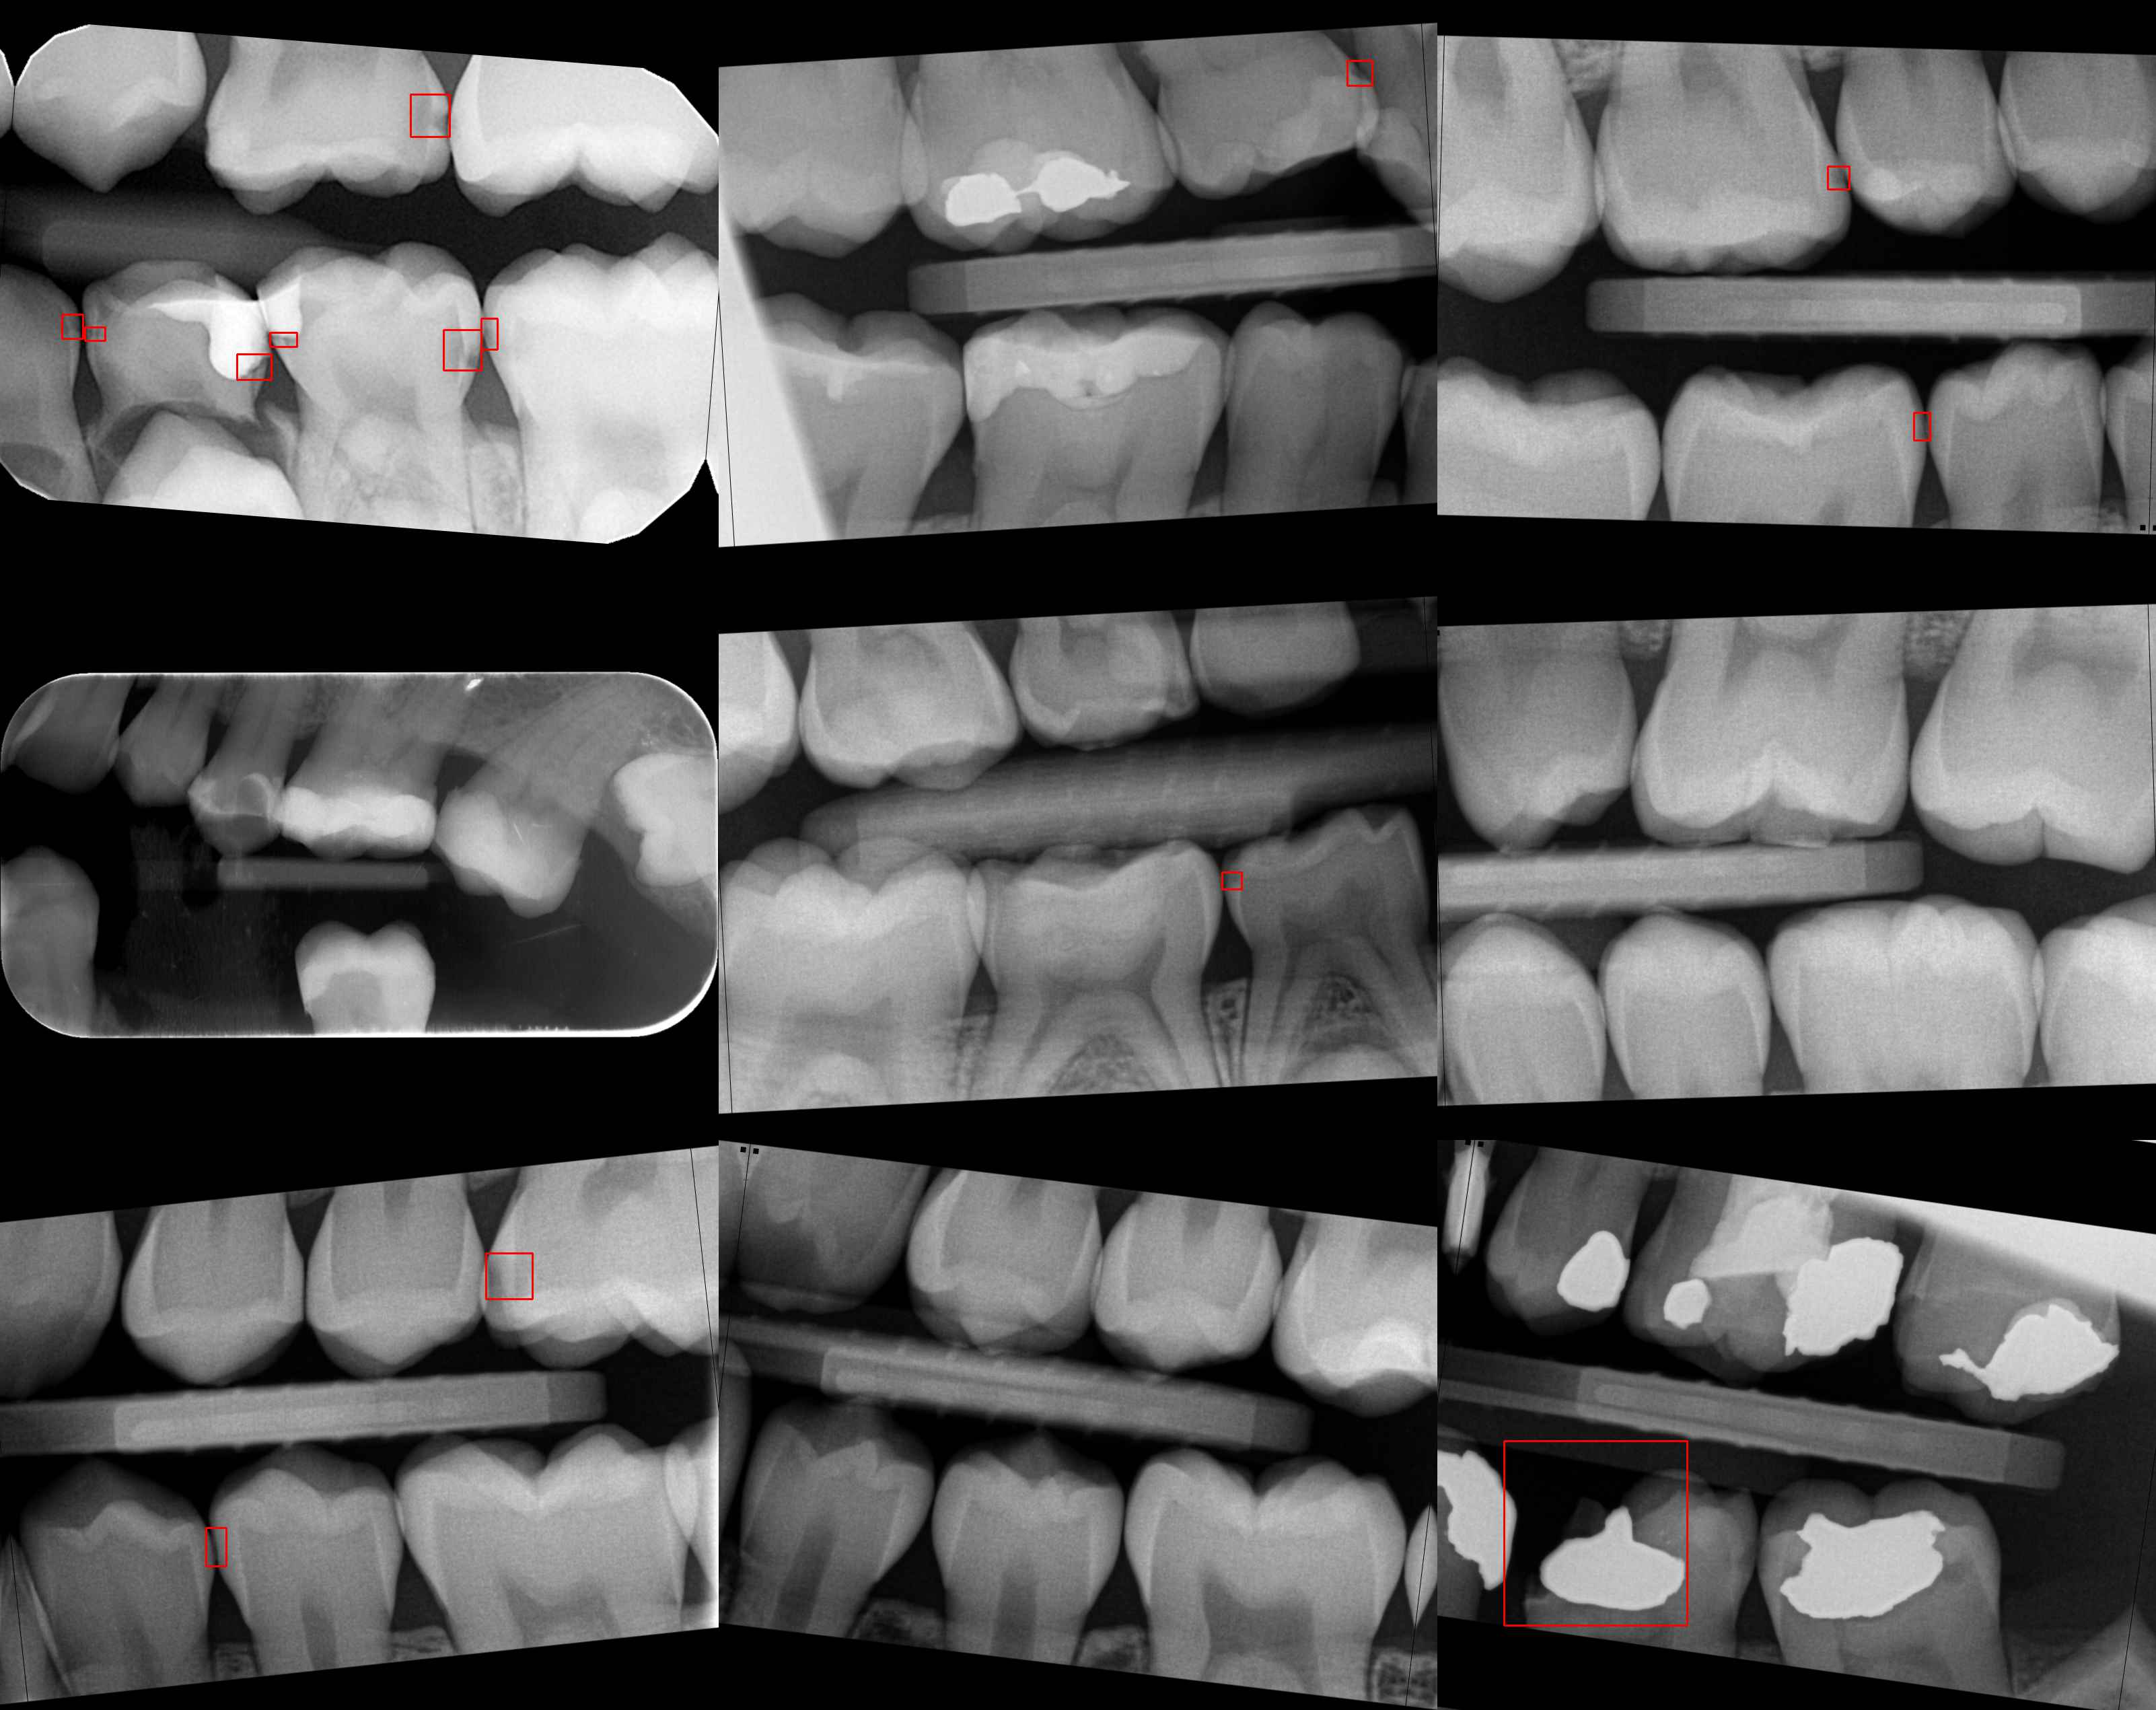
\includegraphics[width =0.9\linewidth]{images/roate_10.jpg}
    \caption{Rotation applied}
\end{figure}
\begin{figure}
    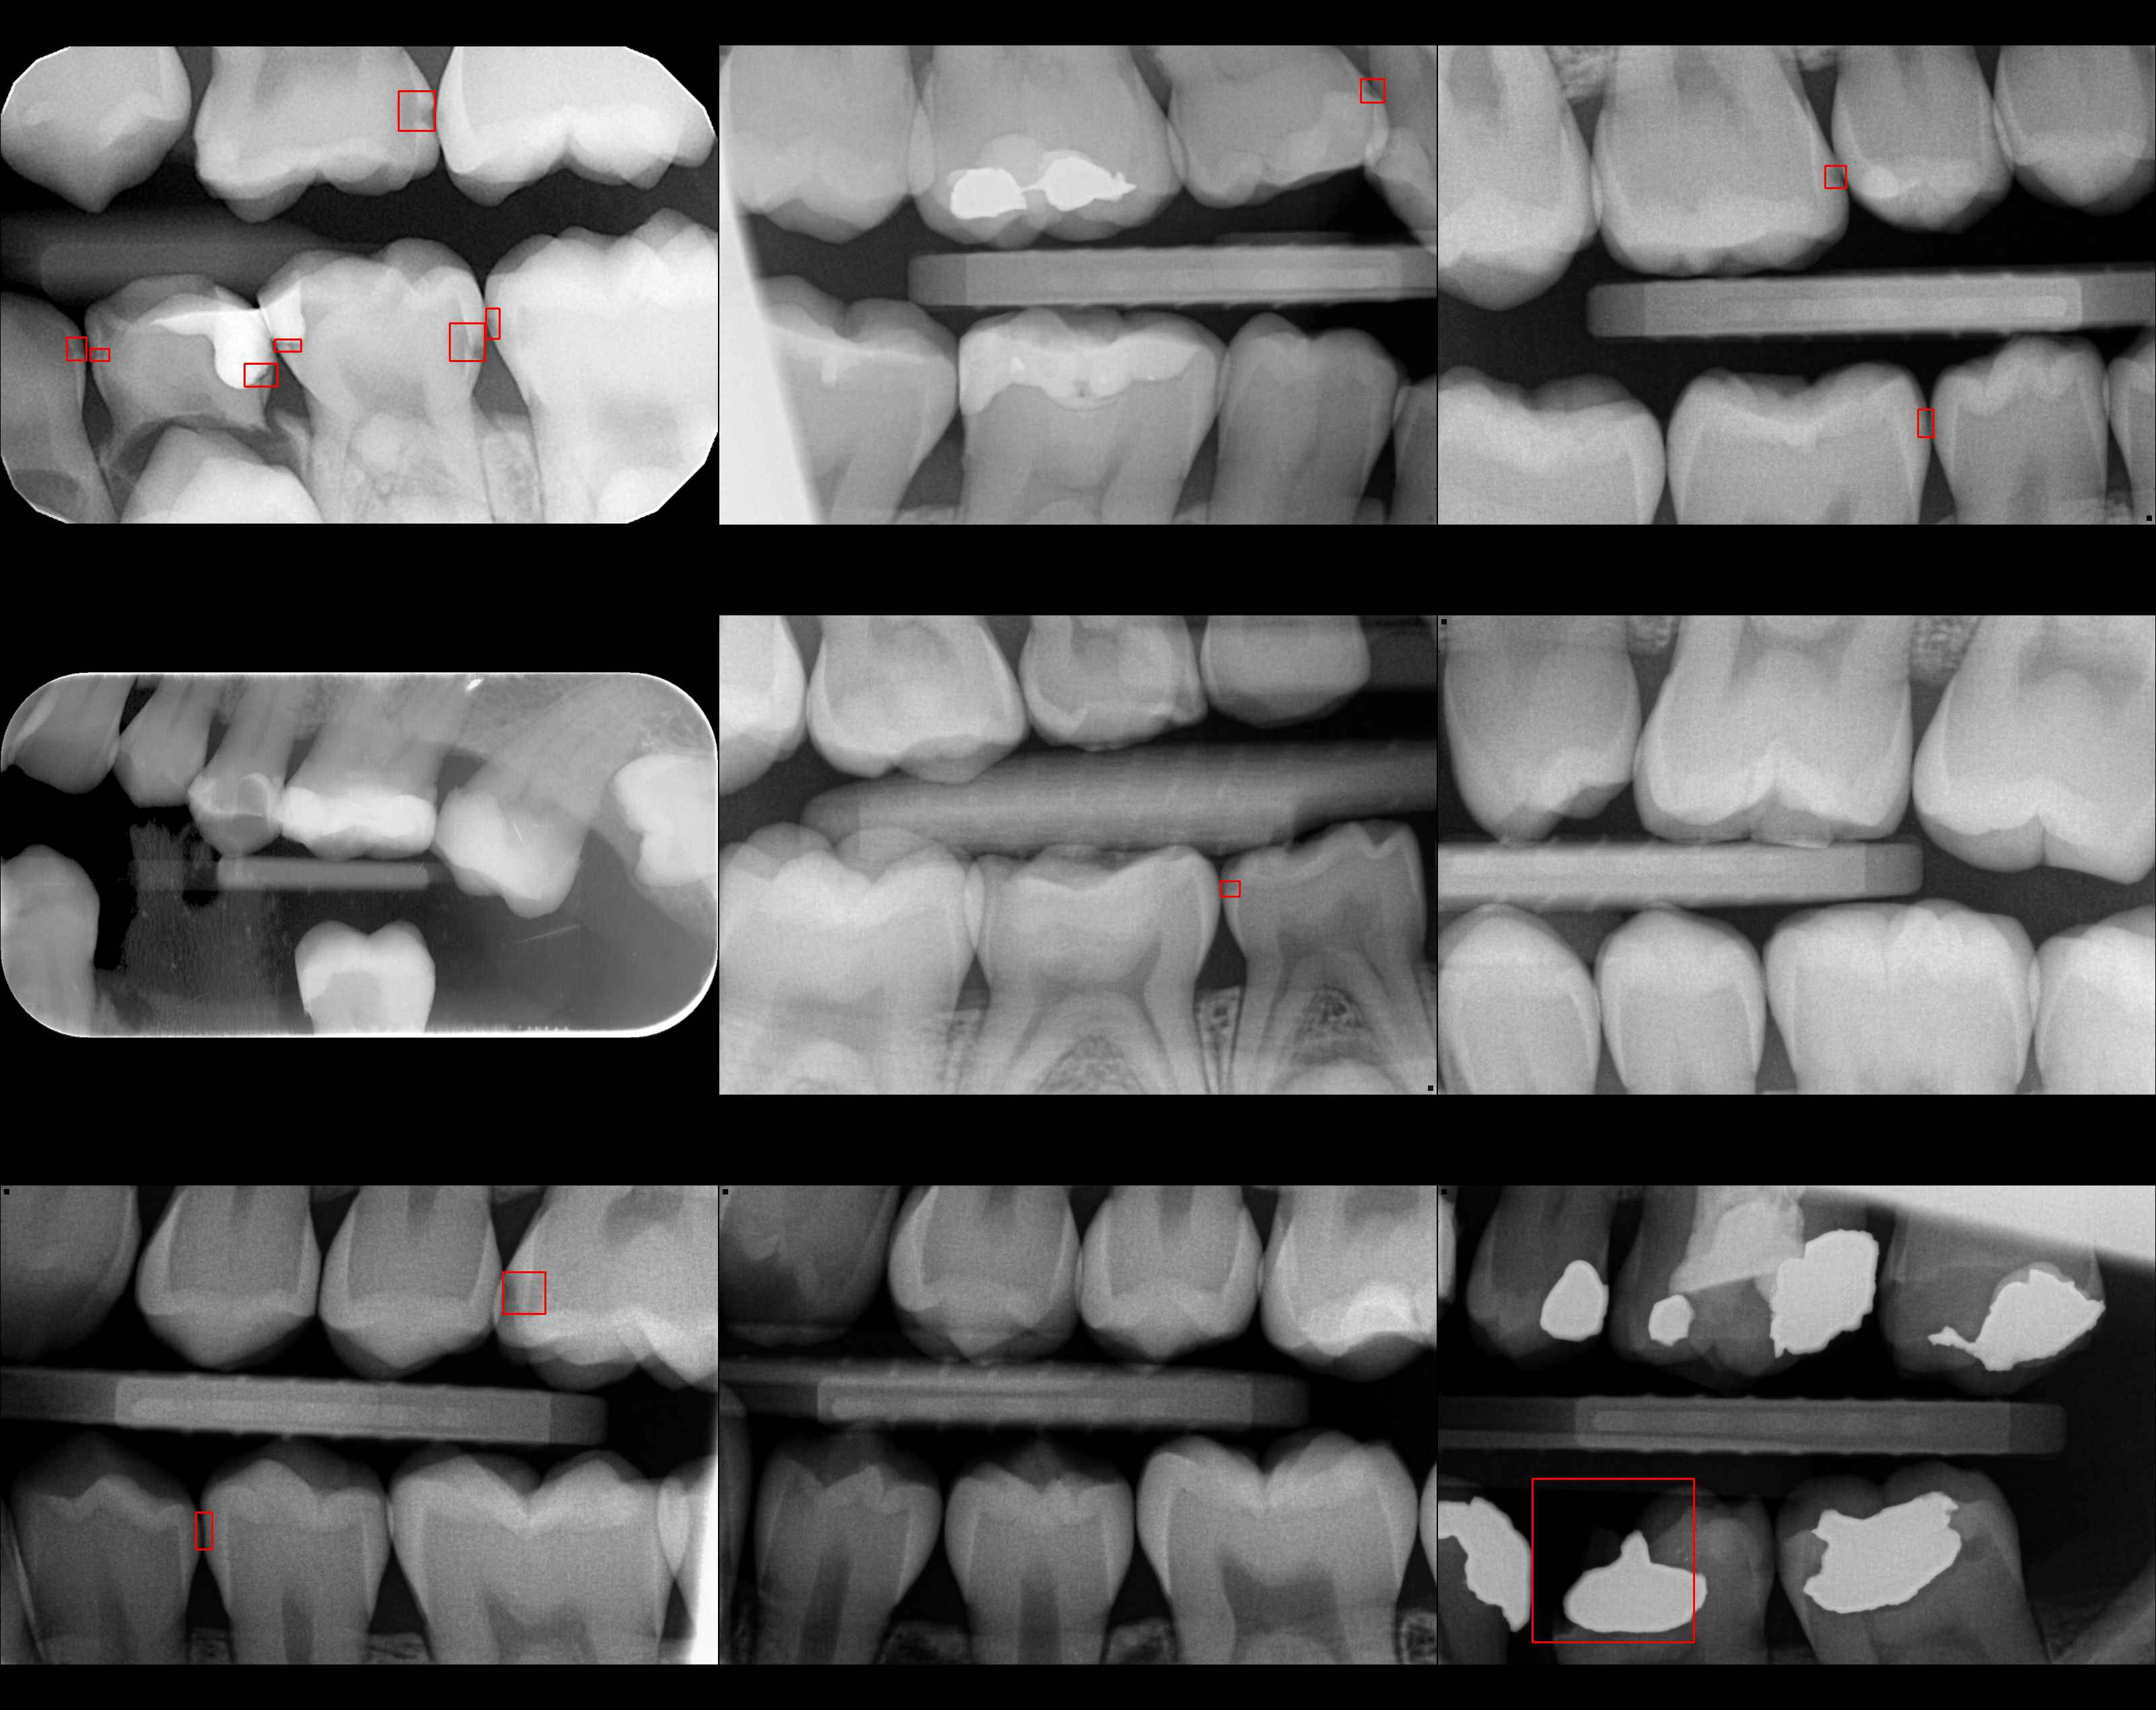
\includegraphics[width =0.9\linewidth]{images/random_gamma.jpg}
    \caption{Gamma correction applied}
\end{figure}
\begin{figure}
    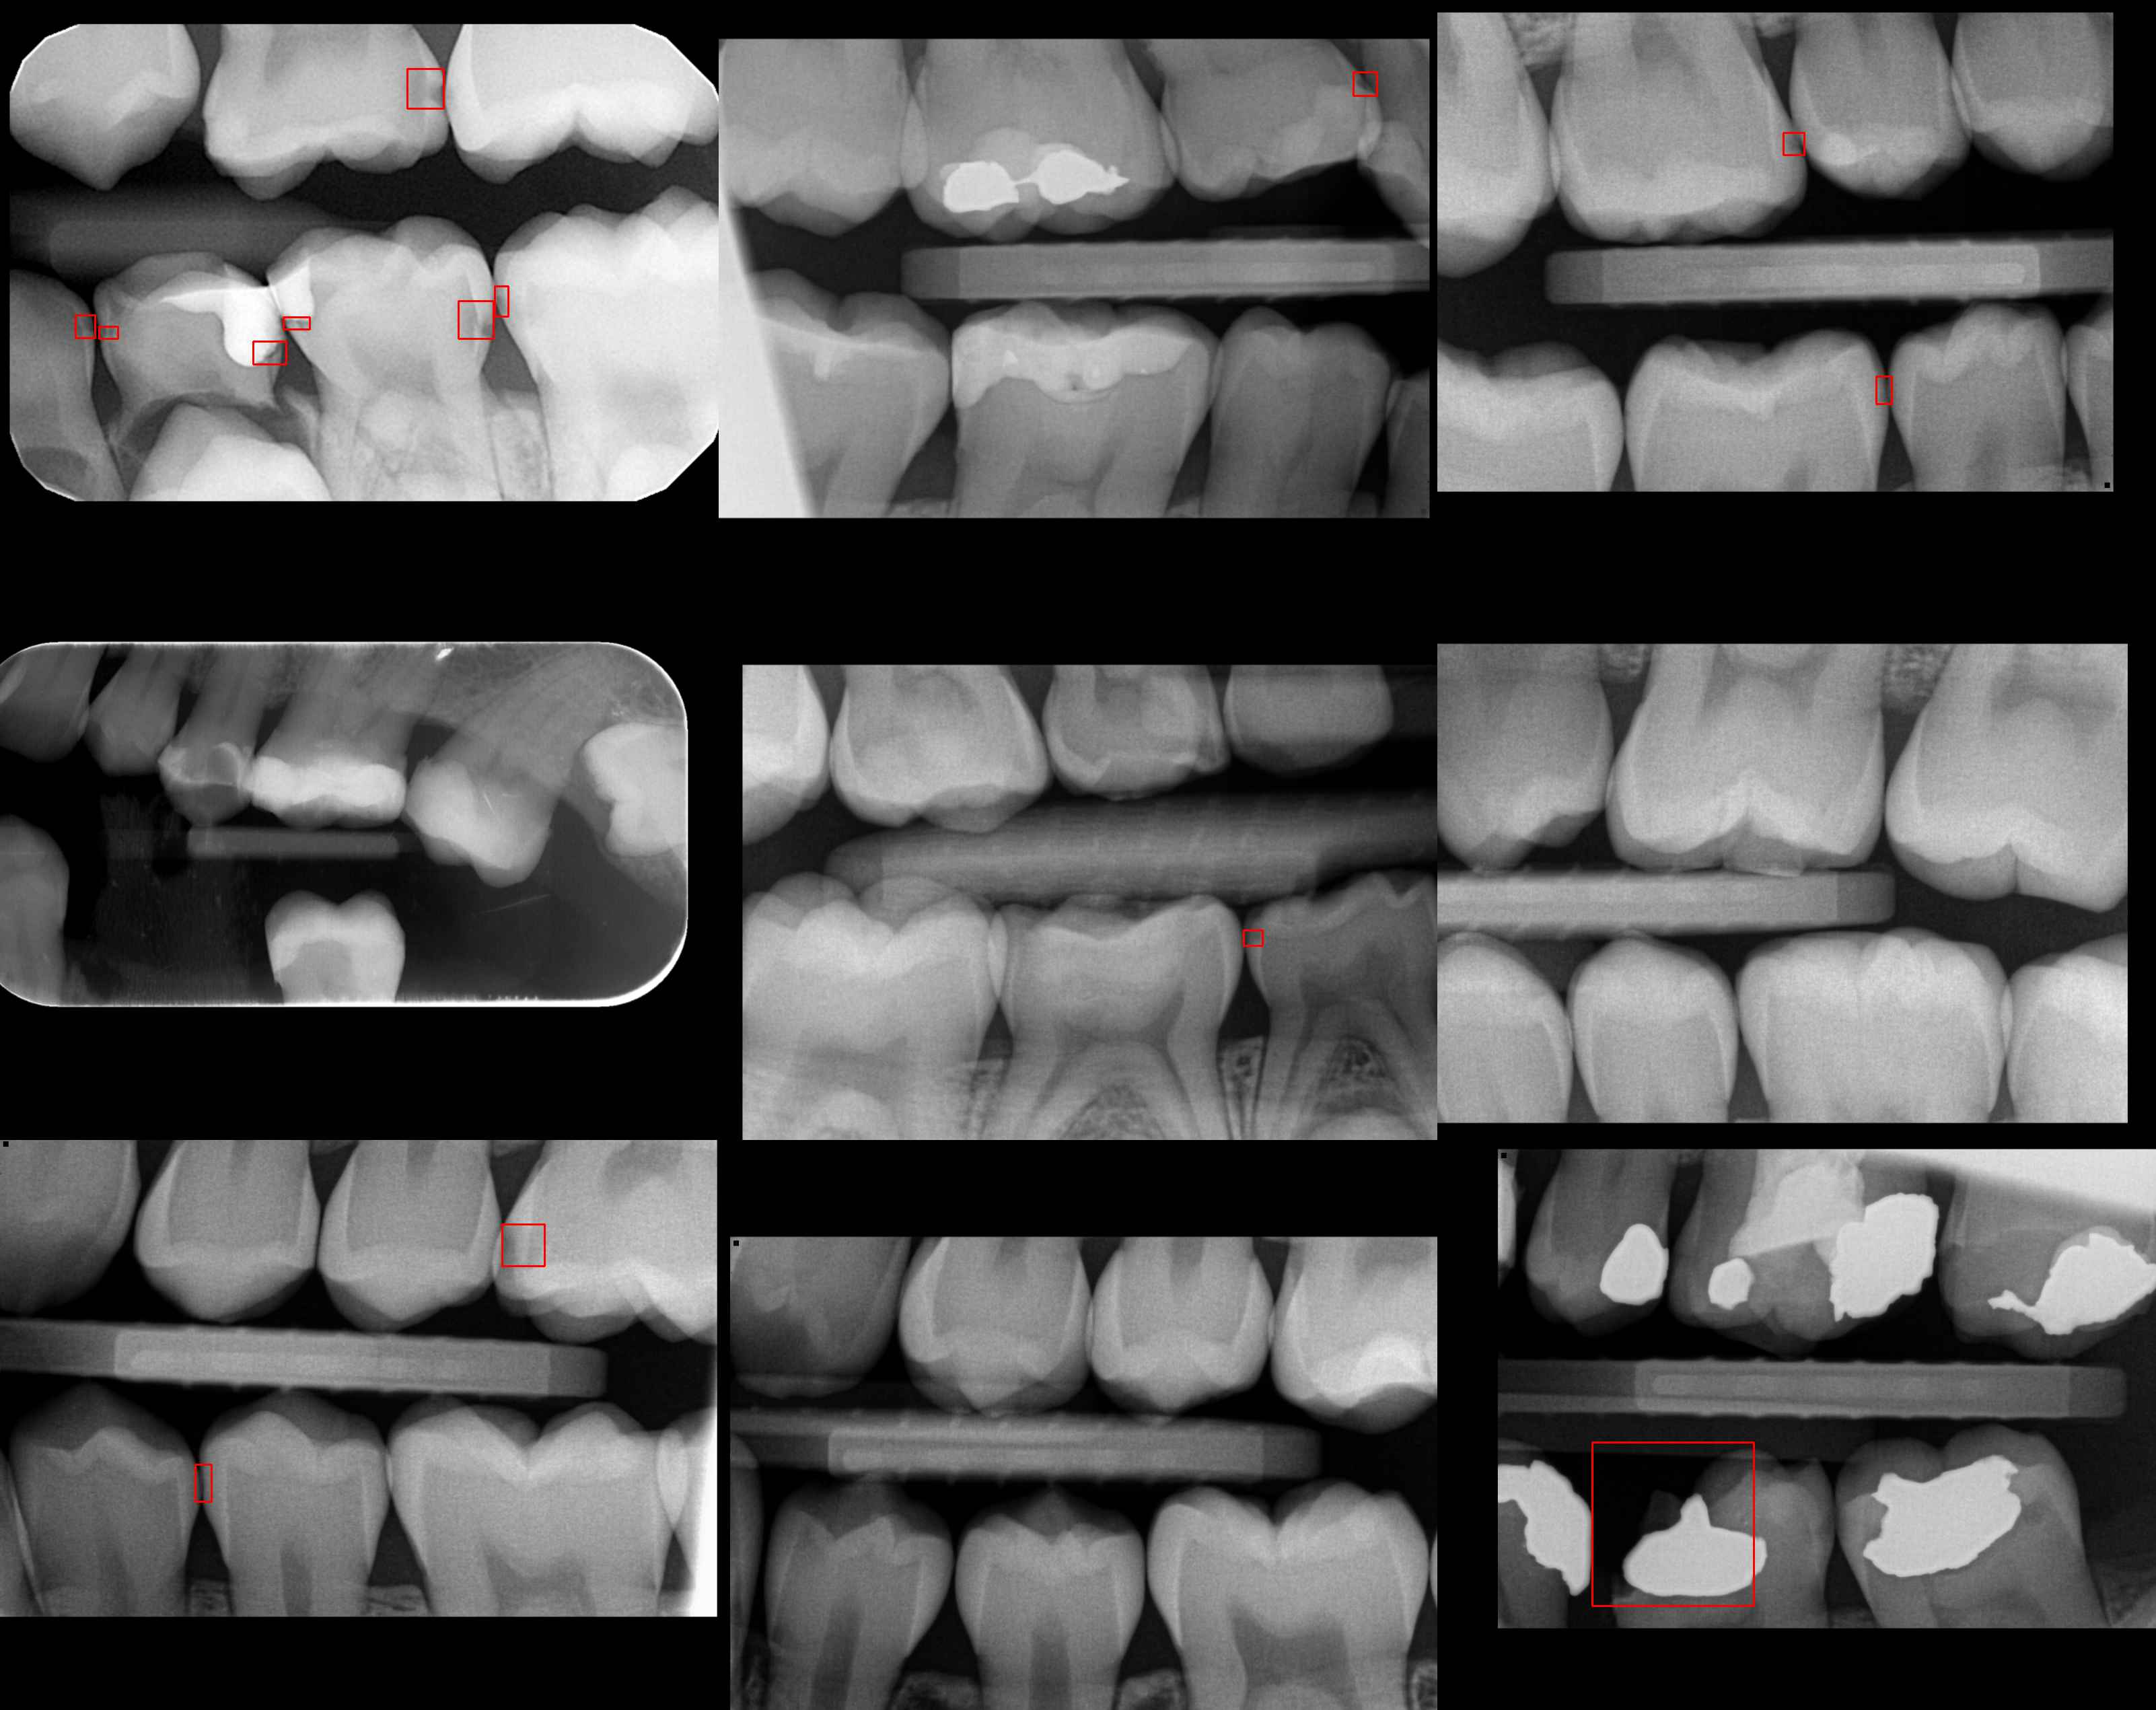
\includegraphics[width =0.9\linewidth]{images/translate.jpg}
    \caption{Translation applied}
\end{figure}
\begin{figure}
    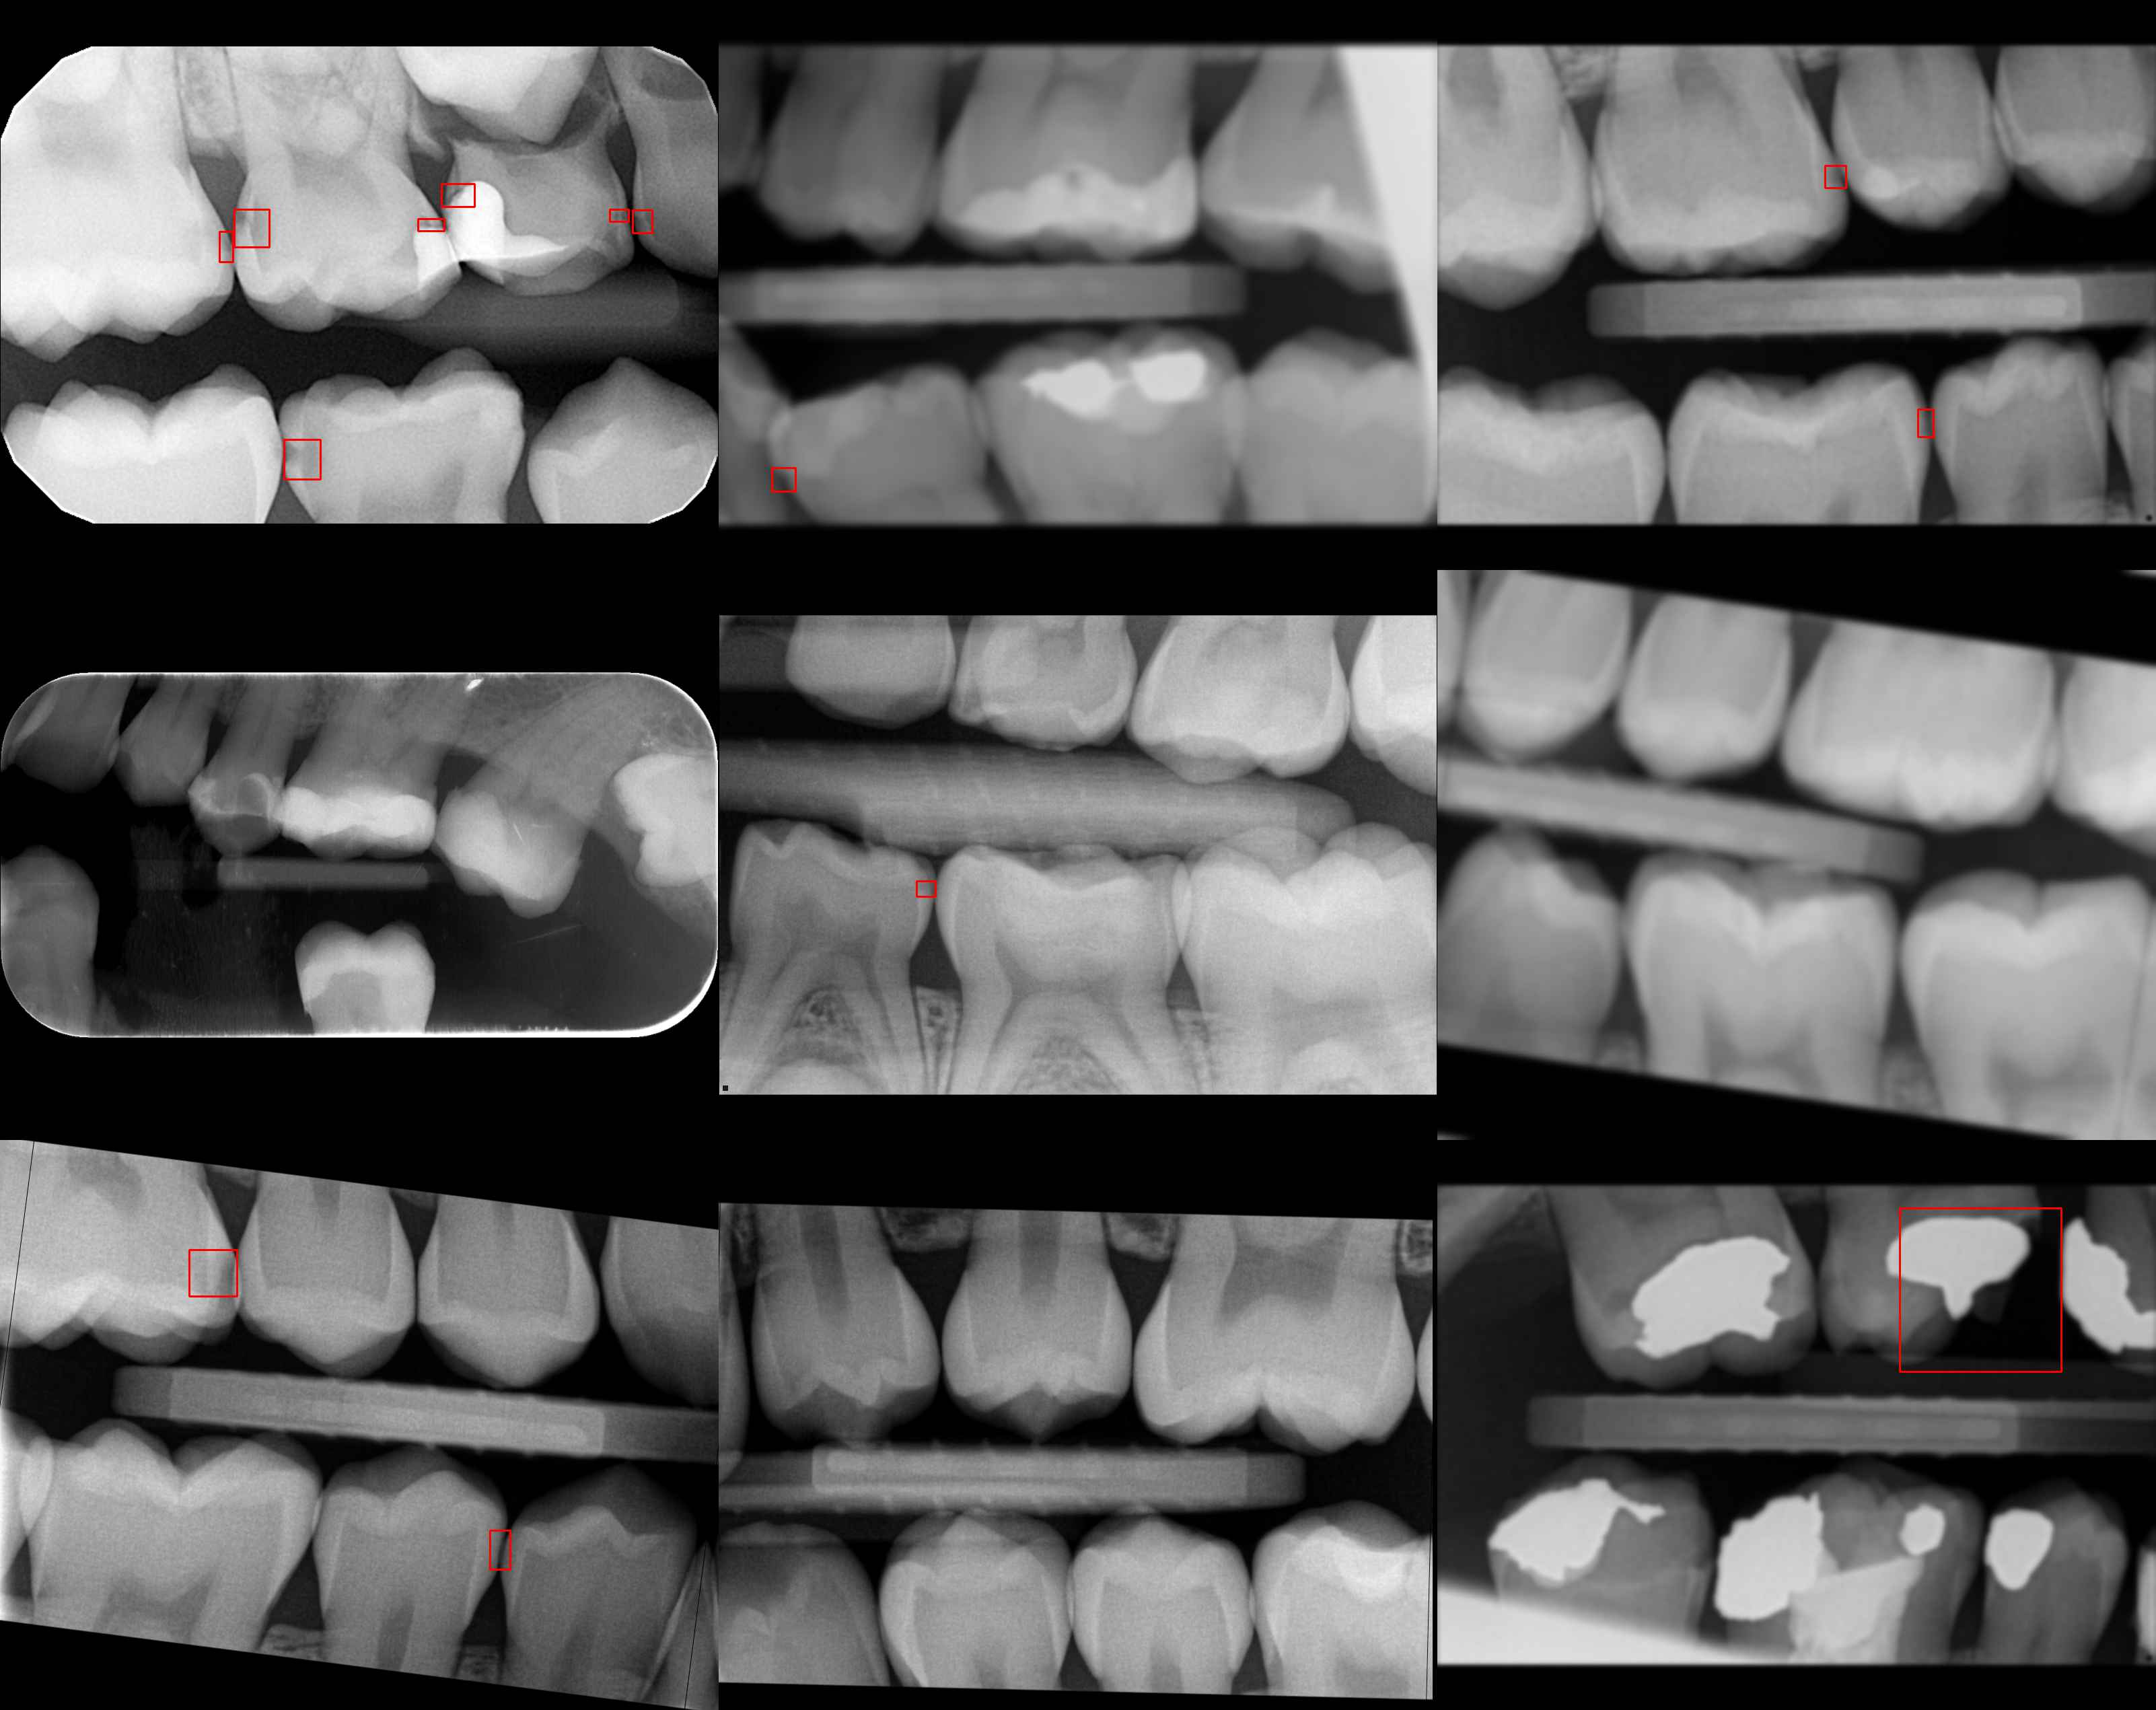
\includegraphics[width =0.9\linewidth]{images/all_transf.jpg}
    \caption{The whole augmentation pipeline applied}
\end{figure}